\section{Spezifikation und Implementierung}
\begin{flushright}
Liviu Beraru
\end{flushright}

\subsection{Spezifikation}
Die Spezifikation der virtuellen Maschine UMach -- dessen Name von
\glqq{}sat\emph{u}rn \emph{mach}ine\grqq{} kommt, da sie als großes entferntes
Ziel wahrgenommen wurde -- umfasst mehrere Themen, die in einem umfangreichen
Dokument behandelt wurden. Das Dokument ist Teil der Abgabe und wird sowohl aus
PDF-Dokument als auch schriftlich dem Projekt-Betreuer übergeben. Die PDF-Datei
heißt \glqq{}UMachVM-Spec.pdf\grqq{}. Der Titel lautet \glqq{}UMach
Spezifikation\grqq. Die Themen dieses Dokumentes werden im folgenden kurz
vorgestellt.


\paragraph{Architektur}
Die Architektur der UMach Maschine orientiert sich stark an der RISC
Architektur. Sie ist registerbasiert und hat eine feste Instruktionslänge von 4
Byte. Die Byte-Reihenfolge ist \glqq{}little endian\grqq{}. Die UMach Maschine
verwendet Port I/O. Es werden 32 Allzweckregister und 13 Spezialregister
definiert. Bestimmte Spezialregister sind schreibgeschützt.



\paragraph{Instruktionssatz}
Es wurden für die UMach-Maschine 69 Instruktionen festgelegt. Für jede
Instruktion wird eine Befehlsnummer, einen Assemblernamen, die Argumente und ein
Instruktionsformat angegeben. Zudem werden für die meisten Instruktionen
Verwendungsbeispiele und Fehlerquellen gegeben. Die Instruktionen werden in
mehreren Kategorien unterteilt: arithmetische, logische, Speicher-, Vergleichs-,
Sprunginstruktionen usw. Die Spezifikation wird nach diesen Kategorien
strukturiert.

Jede Instruktion besteht aus einer Befehlsnummer im ersten Byte und aus
Befehlsargumenten in den folgenden 3 Bytes. Zur Interpretieung der
Instruktionsargumente wurden Instruktionsformate definiert. Gemäß dieser
Formate, können die 3 Argumentenbytes entweder als Registernummer, oder direkte
nummerische Angaben interpretiert werden, die 1, 2 oder 3 Bytes groß sind.


\paragraph{Speichermodell}
Die UMach Maschine verwendet nur absoluten Speicheradressen. Der gesamte
Adressraum wird für den Speicher verwendet (kein Mapping für I/O-Ports). Der
Speicher wird in 5 Segmenten eingeteilt: Interrupttabelle, Code-Segment,
Datensegment, Heap und Stack. Zur Kennzeichnung der Segmentgrenzen dienen
Registerwerte. Ausnahme macht die Interrupttabelle, die die Adressen 0 bis 255
belegt.

Lese- und Schreibeoperationen werden durch geeignete \emph{load}-, 
\emph{store}-, \emph{push}- und \emph{pop}-Instruktionen ausgeführt. Zudem
können die Grenzen der Speichersegmente durch Änderung bestimmter Registerwerte
verändert werden, insbesondere durch die Register \texttt{HE} (heap end) und
\texttt{SP} (stack pointer).


\paragraph{I/O Modell}
Die UMach Maschine verwendet Port I/O, als Gegenteil zu Memory Mapped I/O. Die
Spezifikation beschreibt die Struktur der I/O-Einheit, die für die Eingabe und
Ausgabe verantwortlich ist. Sie beinhaltet 8 Ausgabeports und 8 Eingabeports.
Für Eingabe und Ausgabe werden spezielle \texttt{IN} und \texttt{OUT}
Instruktionen zur Verfügung gestellt. Die aktuelle Implementierung der UMach
Maschine bindet alle Eingabeports an die standard Eingabe (\texttt{stdin}) und
alle Ausgabeports an die standard Ausgabe (\texttt{stdout}).


\paragraph{Interruptmodell}

Für die UMach Maschine wurde ein Interrupt-Mechanismus konzipiert und
entwickelt. Die Spezifikation beschreibt diesen Mechanismus im Detail.
Interrupts sind Signale, die entweder von der Maschine selbst oder vom
Programmierer generiert werden können. Jedem Interrupt wird eine Interruptnummer
vergeben. Von der Maschine werden sie in Fehlerfälle, vom Programmierer werden
die mit der Instruktion \texttt{INT} generiert. Ein Interrupt kann abgefangen
werden indem in der Interrupttabelle die Adresse einer entsprechenden Routine
eingetragen wird.


\subsection{Implementierung}

Die UMach Maschine wurde in C99 implementiert. Das Programm heißt \texttt{umach}
und wurde für Linux bzw. POSIX geschrieben. Beim Start dieses Programms können
verschiedene Argumente übergeben werden. Siehe dazu das Dokument
UMachVM-Verwendung.pdf. 

Das \texttt{umach} Programm besteht aus mehreren Komponenten, die in der
Abbildung \ref{fig:umachstruktur} auf Seite \pageref{fig:umachstruktur}
dargestellt sind. Diese Komponenten sind:

\begin{enumerate}
  \item Maschine: Funktionen und Datenstrukturen, die den Kern, Speicher und
     I/O Einheit der Maschine realisieren. Die I/O Einheit ist nicht in einer
     Code-Datei vorhanden, sondern als Implementierung der I/O-Instruktionen.
     Eine zukünftige Version der UMach-Maschine sollte diese Einheit getrennt
     implementieren.
  \item Disassembler: Ausgabe eines Bytecode-Datei in Assembler-Schreibweise.
  \item Debugger: eingebauter einfacher Debugger.
\end{enumerate}

Der Abschnitt \ref{sec:umach-uebersicht-c-dateien} auf Seite
\pageref{sec:umach-uebersicht-c-dateien} stellt die C-Dateien vor, die diese
Komponenten ausmachen.

\begin{figure}[h!tp]
\centering
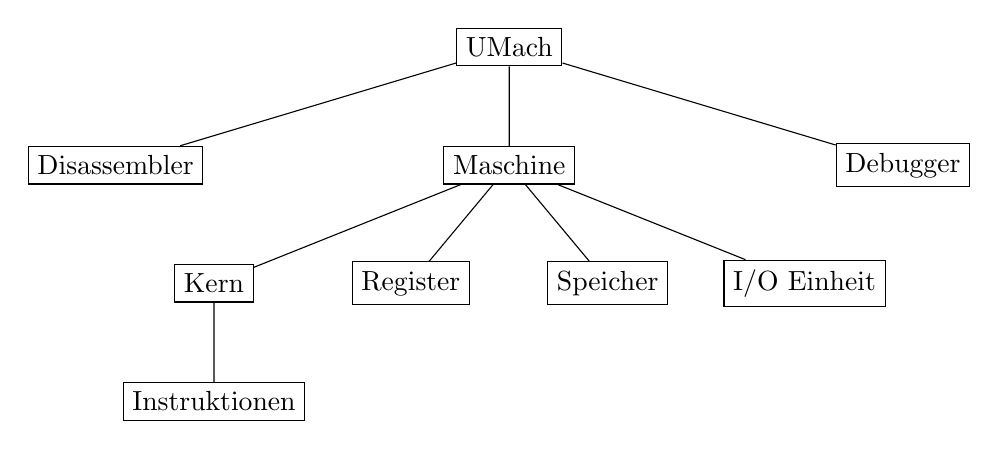
\begin{tikzpicture}
[every node/.style={draw},
 level/.style={sibling distance=5cm/#1}]
\node{UMach}
child
{
    node {Disassembler}
}
child 
{
    node {Maschine}
    child
    { node{Kern}
      child { node{Instruktionen} }
    }
    child { node{Register} }
    child { node{Speicher} }
    child { node{I/O Einheit} }
}
child
{
    node {Debugger}
}
;
\end{tikzpicture}
 

\caption[Struktur des umach Programms]
{Komponenten-Struktur des \texttt{umach} Programms}
\label{fig:umachstruktur}
\end{figure}





\subsubsection{Grundablauf}
Die \texttt{main}-Funktion befindet sich in der Datei umach.c. Das Programm
fängt gewöhnlich damit an, dass der UMach-Speicher gemäß Programmoptionen
initialisiert wird. Dabei wird die Programmdatei, die als Programmargument
übergeben wird, in den Code-Segment geladen und entsprechend die
Segment-Register initialisiert. Danach wird aus \texttt{main} in das Modul
\texttt{core} gesprungen (Datei core.c, Funktion \texttt{core\_run\_program})
und dort innerhalb einer Schleife alle Instruktionen aus dem Code-Segment
ausgeführt. Das Programm stoppt in folgenden Fällen:
\begin{itemize}
  \item Der Wert des Registers \texttt{PC} zeigt in den Datensegment
(überschreitet den Code-Segment).
  \item Die Instruktion \texttt{EOP} (end of programm) wurde ausgeführt.
  \item Ein Interrupt wurde generiert, der von keiner Subroutine abgefangen
wird.
\end{itemize}


Die Ausführung jeder Instruktion hat zwei Schritte, die sich am Von
Neumann Zyklus orientieren:
\begin{enumerate}
  \item fetch: die nächste Instruktion wir aus dem Code-Segment in ein globales
4-bytiges Array geladen. 
  \item execute: die jenige Funktion, die der Befehlsnummer im Byte 0 der
Instruktion entspricht wird ausgeführt. Diese Funktion liest die Argumente aus
dem globalen Array wo die Instruktion geladen wurde. Anschließend wird der Wert
des \texttt{PC} Registers mit 4 inkrementiert.
\end{enumerate}


\subsubsection{Sprungtabelle}

Ein wichtiges Konzept in der Implementierung der UMach Maschine ist die
sogenannte Sprungtabelle. Sie besteht aus einem Array von Strukturen, die nach
einem Schlüssel indiziert wird. Sie ist eine einfache Hashtabelle und wird
verwendet, um die jenige Funktion zu finden, die eine bestimmte Instruktion
implementiert. Schlüssel ist die Befehlsnummer der Instruktion.

Um das Konzept deutlicher zu machen, betrachte man als Beispiel die folgende
Struktur:
\begin{lstlisting}
typedef struct command 
{
    int (*execute) (void);
}
command;
\end{lstlisting}

Sie besteht aus einem einzigen Feld: ein Funktionszeiger namens
\texttt{execute}. Die gezeigte Funktion hat eine bestimmte Signatur: sie nimmt
keine Argumente und gibt ein Integer zurück. Nun kann man eine Sprungtabelle wie
folgt definieren:
\begin{lstlisting}
command opmap[OPMAX] = 
{
  [0x00] = { core_nop },
  [0x04] = { core_eop },
  [0x10] = { core_set },
  [0x11] = { core_cp  },
  [0x12] = { core_lb  },
  [0x13] = { core_lw  },
  [0x14] = { core_sb  },
  [0x15] = { core_sw  },
  ...
  [0xB8] = { core_out }
}
\end{lstlisting}

Alle Funktionsnamen auf der rechten Seite sind Namen von Funktionen, die wir
implementiert haben. Die ausdrückliche Index-Zuweisung gehört zum C99-Standard
und war einer der Gründe, warum C99 für dieses Projekt ausgewählt wurde. Möchte
man jetzt die Instruktion mit Nummer \texttt{0x13} ausführen, so schaut man in
dieser Tabelle (Array) am Index \texttt{0x13} nach und falls der Eintrag nicht
Null ist, führt man die Funktion aus:

\begin{lstlisting}
command cmd = opmap[0x13];
if (cmd.execute) {
    cmd.execute();
}
\end{lstlisting}

Nach diesem Prinzip funktioniert der Kern der UMach Maschine, bzw. die Funktion
\texttt{core\_execute}, die den \glqq{}execute\grqq{}-Schritt implementiert und
in der Datei core.c definiert ist. Die \texttt{command}-Struktur, die hier
vereinfacht wurde, wird in der Datei command.h definiert, die Sprungtabelle
selbst in command.c. Dort enthält die \texttt{command}-Struktur Felder für das
Instruktionsformat, Name der Instruktion etc, die vom Assembler und Disassembler
verwendet werden.

Diese Sprungtabelle ist eine Art, den \glqq{}command pattern\grqq{} in C zu
implementieren.


\subsubsection{Registertabelle}

Für die Register der Maschine wurde ein ähnliches Konzept wie für die
Sprungtabelle der Instruktionsfunktionen verwendet: eine Tabelle (Array) von
Strukturen, die nach Registernummern indiziert wird. Die entsprechende Struktur
\texttt{register} wird in der Datei register.h definiert und enthält Felder für
den Registerwert, Zugriffsrechte und für den Registernamen, der vom Disassembler
gebraucht wird. Um den Wert eines Registers mit Nummer $x$ zu setzen, adressiert
man die Tabelle an Index $x$ und setzt das entsprechende Feld.



\subsubsection{Übersicht der C Dateien}
\label{sec:umach-uebersicht-c-dateien}

Die Implementierung erstreckt sich über 38 Dateien, die man wie folgt
gruppieren kann:

\paragraph{Main}
Die \texttt{main} Funktion befindet sich in umach.c. Hier werden
Programmargumente eingelesen, der UMach-Speicher initialisiert und das Programm
in den Code-Segment geladen. Dann wird zum Modul \texttt{core} gesprungen und
das Programm ausgeführt.

\paragraph{Kern}
Die Funktionen, die zum Kern (\texttt{core}) der UMach-Maschine gehören, sind in
der Datei core.c implementiert und in der Headerdatei core.h deklariert. Dazu
zählen Funktionen, die die Schritten fetch und execute implementieren. Hier
findet man auch das globale Array \texttt{instruction}, das die aktuelle
Instruktion enthält und den Integer \texttt{running}, der 0 wird, wenn die
Maschine hält, sonst immer 1 ist. Die Funktion \texttt{core\_run\_program} führt
die Schritte fetch und execute solange aus, bis die Variable \texttt{running} 0
wird.

\paragraph{Speicher}
Der Speichermodull (Dateien memory.c und memory.h) enthält Funktionen zum
Speicher initialisieren und freigeben, Speicher lesen und schreiben, Laden der
Programmdatei in den Code-Segment, und Funktionen, die die Befehle
\texttt{PUSH} und \texttt{POP} realisieren.

\paragraph{Register}
Die Dateien register.c und register.h enthalten die Registertabelle und
Funktionen zum Lesen und Schreiben der Registerinhalte und zum Setzen einzelner
Bits in Registern. Zusätzlich werden Registernummern definiert.

\paragraph{Instruktionen}
Die UMach-Instruktionen werden in Kategorien unterteilt: arithmetische
Instruktionen, logische Instruktionen usw. Diese Kategorien werden in der
Spezifikation eingeführt. Für jede Kategorie von Instruktionen, wird eine
getrennte C-Datei und Headerdatei verwendet. In dieser Datei werden alle
Instruktionen implementiert, die der entsprechenden Kategorie gehören. Alle
diese Funktionen wurden nach demselben Muster benannt: \glqq{}core\_$x$\grqq{}.
Wobei $x$ ist der Assemblername der Instruktion, so wie in der Spezifikation
festgelegt. Beispiele wären \glqq{}core\_add\grqq{}, \glqq{}core\_sub\grqq{},
\glqq{}core\_jmp\grqq{} usw.

Möchte man also den Quellcode einer bestimmten Instruktion $\iota$ finden, so
schaut man in der Spezifikation, zu welcher Kategorie $\kappa$ gehört die
Instruktion $\iota$. Dann schaut man in der C-Datei zur Kategorie $\kappa$ nach
einer Funktion mit dem Namen \glqq{}core\_$\iota$\grqq{}. Zum Beispiel die
Instruktion \texttt{ADD} ist in der Kategorie \glqq{}Arithmetische
Instruktionen\grqq{}, also schaut man in der Datei arithm.c nach einer Funktion
core\_add.

Hier eine Liste der Dateien:

\begin{center}
\begin{tabular}{ll}
C-Datei      & Kategorie von Instruktionen \\
\hline\hline
controll.c   & Kontrollinstruktionen       \\
loadstore.c  & Lade- und Speicherbefehle   \\
arithm.c     & Arithmetische Instruktionen \\
logic.c      & Logische Instruktionen      \\
compare.c    & Vergleichsinstruktionen     \\
branch.c     & Sprungbefehle               \\
subroutine.c & Unterprogramminstruktionen  \\
system.c     & Systeminstruktionen         \\
io.c         & IO Instruktionen            \\
\hline
\end{tabular}
\end{center}

Zu jeder C Datei gehört eine Headerdatei gleichen Namens, die hier nicht mehr
gezeigt wurde. Die Wörter \glqq{}Instruktion\grqq{} und \glqq{}Befehl\grqq{}
werden in der Benennung der einzelnen Kategorien gleichgesetzt.

\paragraph{Interruptnummern}
Die Interruptnummern sind in der Headerdatei interrupts.h deklariert.



\paragraph{Disassembler}
Die Dateien disassemble.c und disassemble.h enthalten die Implementierung eines
einfachen Disassemblers. Der Disassembler liest eine Datei Instruktion für
Instruktion aus, disassembliert jede davon und gibt sie auf die standard
Ausgabe aus. Der Disassembler stoppt wenn er entweder die Datei bis zu Ende
gelesen hat, oder wenn er eine spezielle Marke (Bytemuster) einliest, die den
Start des Datensegments signalisiert. Diese Marke wird vom Assembler am Ende
des Code-Segments geschrieben und wird auch vom Speicher-Modull verwendet, um
das Ende dieses Segments zu erkennen.

\paragraph{Debugger}
Die UMach Maschine besitzt einen eingebauten einfachen Debugger, der in den
Dateien debugger.c und debugger.h implementiert wird. Der Debugger zeigt immer
eine disassemblierte Instruktion und wartet auf einen Befehl vom Benutzer. Nach
der Ausführung einer Funktion wartet zeigt er die nächste Instruktion und
wartet auf einen neuen Befehl. Der Debugger benutzt den Disassembler-Modull um
die einzelnen Instruktionen zu disassemblieren. Seine Verwendung wird in der
Dokumentationsdatei UMachVM-Verwendung.pdf beschrieben.

\paragraph{Optionen}
Die Dateien options.h und options.c deklarieren eine Optionenstruktur, die die
Programmoptionen enthält. Sinn davon ist, dass diese Optionen an mehreren
Stellen in Programm verwendet werden, was eine globale Deklaration notwendig
macht. Die Optionen werden in umach.c gesetzt, wenn die Programmargumente
ausgelesen werden.

\paragraph{Logging}
Das Modul \texttt{logmsg} (Dateien logmsg.c und logmsg.h) enthält ein einfaches
Mechanismus zur bedingten Ausgabe von Nachrichten. Jede Nachricht wird dem Modul
mit einem \glqq{}level\grqq{} übergeben. Je nach Wert des Feldes
\texttt{verbose} in der Optionenstruktur, wird die Nachricht ausgegeben oder
nicht.

\paragraph{Utils}
Die Datei strings.c enthält ein paar nützliche Funktionen zur Bearbeitung von
Zeichenketten: zersplittern, Leerzeichen überspringen und Zahlen parsen.

\paragraph{Makefile}
Das Makefile dient zur Kompilierung des \texttt{umach} Programms. Man kann das
Programm kompilieren, indem man in das Quellenverzeichniss wechselt und dort
\texttt{make} Eingibt.

